\documentclass[tikz,border=10pt]{standalone}
\usepackage{tikz}
\usetikzlibrary{calc} 
\usetikzlibrary{positioning, fit, arrows.meta, shapes}

% used to avoid putting the same thing several times...
% Command \empt{var1}{var2}
\newcommand{\empt}[2]{$#1^{\langle #2 \rangle}$}

\begin{document}

 
    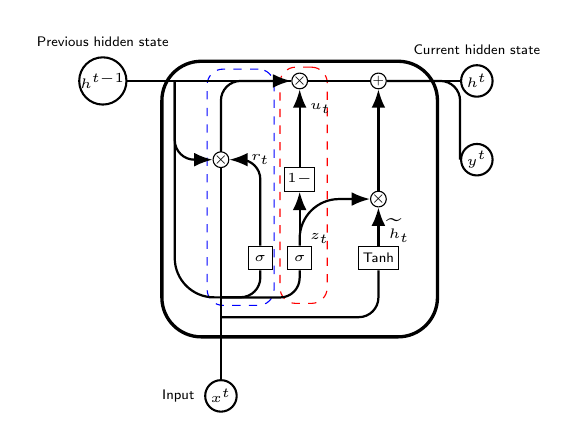
\begin{tikzpicture}[
        font=\sf \tiny,
        >=LaTeX,
        % Styles
        cell/.style={% For the main box
            rectangle, 
            rounded corners=5mm, 
            draw,
            very thick,
            },
        cell2/.style={% For the main box
        rectangle, 
        rounded corners=2mm, 
        draw,
        thin,
        },
        operator/.style={% For operators like +  and  x
            circle,
            draw,
            inner sep=-0.5pt,
            minimum height =.2cm,
            },
        function/.style={% For functions
            ellipse,
            draw,
            inner sep=1pt
            },
        ct/.style={% For external inputs and outputs
            circle,
            draw,
            line width = .75pt,
            minimum width=1cm,
            inner sep=0pt,
            },
        gt/.style={% For internal inputs
            rectangle,
            draw,
            minimum width=3mm,
            minimum height=3mm,
            inner sep=1pt
            },
        mylabel/.style={% something new that I have learned
            font=\tiny\sffamily
            },
        ArrowC1/.style={% Arrows with rounded corners
            rounded corners=.25cm,
            thick,
            },
        ArrowC2/.style={% Arrows with big rounded corners
            rounded corners=.5cm,
            thick,
            },
        ]
    
    % Nodes    
        % Draw the cell boundary: 
        \node [cell, minimum height=3.5cm, minimum width=3.5cm] at (0,0){} ;
        \node [dashed, red, cell2, minimum height=3cm, minimum width=0.6cm] at (0.05,0.175){} ;
        \node [dashed, blue, cell2, minimum height=3cm, minimum width=0.85cm] at (-0.75,0.15){} ;
    
        % Draw inputs named ibox#
        \node [gt] (sigma1) at (-0.5,-0.75) {$\sigma$};
        \node [gt] (sigma2) at (0,-0.75) {$\sigma$};
        \node [gt, minimum width=0.5cm] (tanh) at (1,-0.75) {Tanh};
        \node [gt] (oneminus) at (0,0.25) {$1-$};
    
       % Draw operators named mux# , add# and func#
        \node [operator] (mux1) at (-1,0.5) {$\times$};
        \node [operator] (add1) at (1,1.5) {+};
        \node [operator] (mux2) at (1,0) {$\times$};
        \node [operator] (mux3) at (0,1.5) {$\times$};
    
        % Draw External inputs named as basis h,x
        \node[ct, label={[mylabel]Previous hidden state}, align=center, inner sep=0pt, minimum size=4mm] (h) at (-2.5,1.5) {$h^{t-1}$};
        \node[ct, label={[mylabel]left:Input}, align=center, inner sep=0pt, minimum size=4mm] (x) at (-1,-2.5) {$x^{t}$};
    
        % Draw External outputs named as basis h2,y2
        \node[ct, label={[mylabel]Current hidden state}, align=center, inner sep=0pt, minimum size=4mm] (h2) at (2.25,1.5) {$h^{t}$};
        \node[ct, label={[mylabel]}, align=center, inner sep=0pt, minimum size=4mm] (y2) [below of= h2] {$y^{t}$};
    
    % Start connecting all.
        % Intersections and displacements are used. 
        % Drawing arrows    
        \draw [ArrowC1] (h) -- (mux3) -- (add1) -- (h2);
        \draw [ArrowC1] (add1) coordinate[auto] -|(y2.west);
    
        % Inputs
        \draw [ArrowC1] (x) -- coordinate[auto] (link1) (mux1); 
        \draw [ArrowC1] (x -| sigma2)++(-1,1.25) -| (sigma2);
        \draw [ArrowC1] (x -| tanh)++(-2,1) -| (tanh);
        \draw [ArrowC1] (x.north)++(0,1.04) -| (sigma1.south); 
        \draw [->, ArrowC1] (mux1) ++(0,0.1) |- (mux3) ;
        \draw [->,ArrowC1] (h.east)++(0.6,0) |- (mux1.west);
        \draw [->, ArrowC1] (sigma1.north) |- coordinate[auto]  node[pos=0.5] {$r_t$} (mux1.east);
    
        % Internal
        \draw [->, ArrowC2] (sigma2) |- (mux2);
        \draw [->, ArrowC2] (tanh) -- node[pos=0.4, right] {$\widetilde{h}_t$}(mux2);
        \draw [->, ArrowC2] (oneminus) -- coordinate[auto] node[pos=0.75, right] {$u_t$} (mux3);
        \draw [->, ArrowC2] (sigma2)++(0,0.25) -| node[pos=0.4, right] {$z_t$} (oneminus);
        \draw [->, ArrowC2] (mux2) -- (add1);
        \draw [ArrowC2] (h.east)++(0.6,0) |- ($(x.north)!0.775!(link1)$);
        % \draw[->, ArrowC2] (h.east)++(0.25,0) to [out=0,in=100, looseness=0.85] ($(x.north)!0.2!(h.east)$);
    
    \end{tikzpicture}

\end{document}